\documentclass{MALEO_report}
\usepackage{booktabs}\usepackage{graphicx}\usepackage{placeins}
\title{Volleyball Match Statistics}
\subtitle{L.079.05829 Case Study -- Exercise 1}
\author{Indudhara Swamy Vivekananda (4106839) \and Sanjana Basoor Hemanth Kumar (4108160) \and Rohit Mamgin (4086896)}
\authorrunning{Vivekananda, Kumar, and Mamgin}
\institute{Paderborn University, Germany}
\begin{document}\raggedbottom\emergencystretch=1em
\maketitle
\vspace*{-0.5cm}\begin{center}
\includegraphics[width=2.4cm]{MALEO-logo.png}\end{center}
\section{Tasks 1--4: Data preparation and missingness}
The semicolon-delimited data contain 116 matches and 29 substantive variables; the unnamed first field is a row index and was removed. Date was converted to \texttt{Date}. Missing values occur only in \texttt{Receptions.Home} (23; 19.8\%), both fourth-set fields (44; 37.9\%), and both fifth-set fields (85; 73.3\%). All other variables are complete.
\begin{table}[!htbp]\centering\small
\begin{tabular}{lrrll}\toprule
Variable & Missing & \% & Mechanism & Treatment \\
\midrule
Receptions.Home & 23 & 19.8 & Plausibly MCAR & Median = 74 \\
Set4.Home / Away & 44 each & 37.9 & Structural & 0 = not played \\
Set5.Home / Away & 85 each & 73.3 & Structural & 0 = not played \\
All remaining columns & 0 & 0.0 & Complete & None \\
\bottomrule\end{tabular}
\caption{Missingness classification and imputation decisions.}
\end{table}
The set-score omissions are structural: a fourth set does not exist after a 3--0 result, and a fifth set exists only after a 2--2 set score. Their zeros therefore mean ``not played'' and must not be analysed as genuine set scores. Home receptions are plausibly MCAR: Monte Carlo chi-squared tests found no association with home team ($p=.732$) or away team ($p=.998$), and Wilcoxon tests found no association with observed home points, digs, or kills (all $p>.36$). MCAR cannot be proven from observed data, but accidental recording loss is the most economical explanation. The 23 missing values were replaced by the observed median of 74. The completed data passed an explicit zero-missing-values assertion.

Finally, \texttt{Home.Win} equals one when \texttt{Winner == Home.Team}, otherwise zero. Only 43 of 116 home-designated teams won (37.1\%). An exact two-sided binomial test against 50\% yields $p=.0068$, so the label does not provide evidence of home advantage; tournament scheduling and team strength may confound the result.

\section{Task 5: Normality assessment}
Home total points were selected because they summarize match scoring. The 116 complete observations range from 45 to 112 points (range 67), with mean 85.29, median 88.5, and interquartile range 69--102.25. The QQ plot shows curvature and tail departures from the normal reference line (Figure~\ref{fig:qq}). Shapiro--Wilk gives $W=.930$, $p=1.31\times10^{-5}$; normality is therefore rejected at $\alpha=.05$.
\begin{figure}[!htbp]\centering
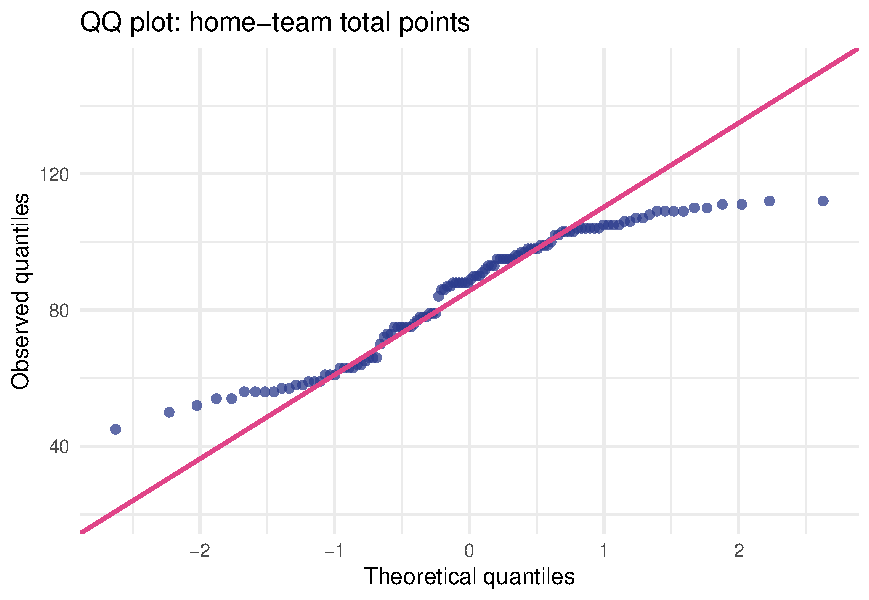
\includegraphics[width=.52\textwidth]{../../outputs/exercise1/qq_total_points_home.pdf}
\caption{QQ plot of home-team total points.}\label{fig:qq}
\end{figure}

\section{Task 6: Exploratory analysis}
Away teams averaged more kills (49.96 versus 47.97), aces (5.15 versus 4.36), digs (60.46 versus 58.41), and total points (89.34 versus 85.29); blocks were practically equal (8.22 versus 8.07). Paired Wilcoxon tests confirm away-side differences for kills ($p=.0046$) and total points ($p=.00029$), but not blocks ($p=.716$). Aces ($p=.052$) and digs ($p=.056$) are borderline, despite paired $t$-test values below .05, and are therefore not treated as robust findings.
\begin{figure}[!htbp]\centering
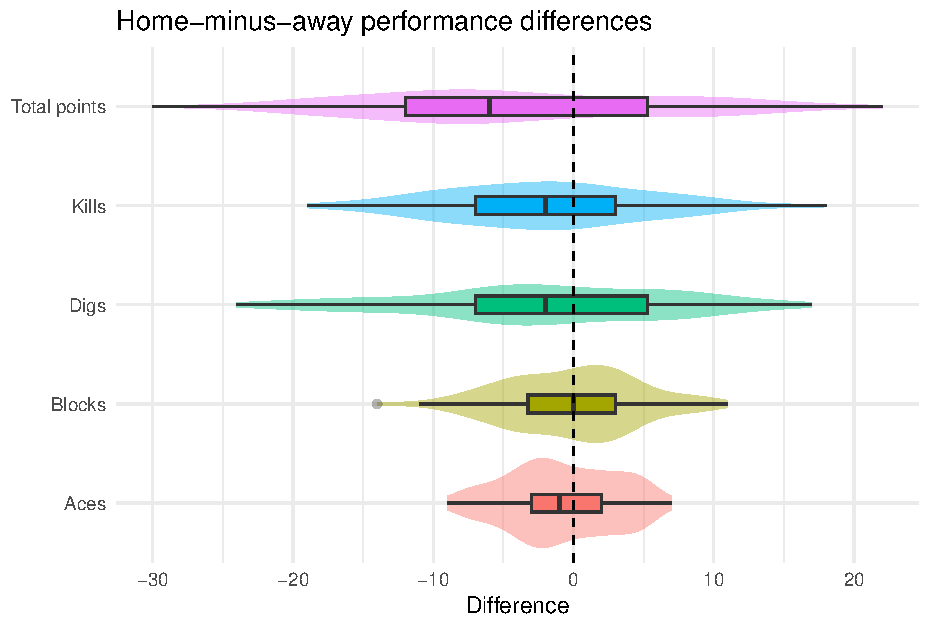
\includegraphics[width=.60\textwidth]{../../outputs/exercise1/home_away_differences.pdf}
\caption{Within-match home-minus-away differences; zero denotes equality.}\label{fig:diff}
\end{figure}
Kills have the clearest linear association with total points ($r=.896$ when both sides are pooled), whereas blocks and aces occupy narrower ranges (Figure~\ref{fig:components}). This result is descriptive, not causal: longer matches generate more opportunities for both kills and total points.
\begin{figure}[!htbp]\centering
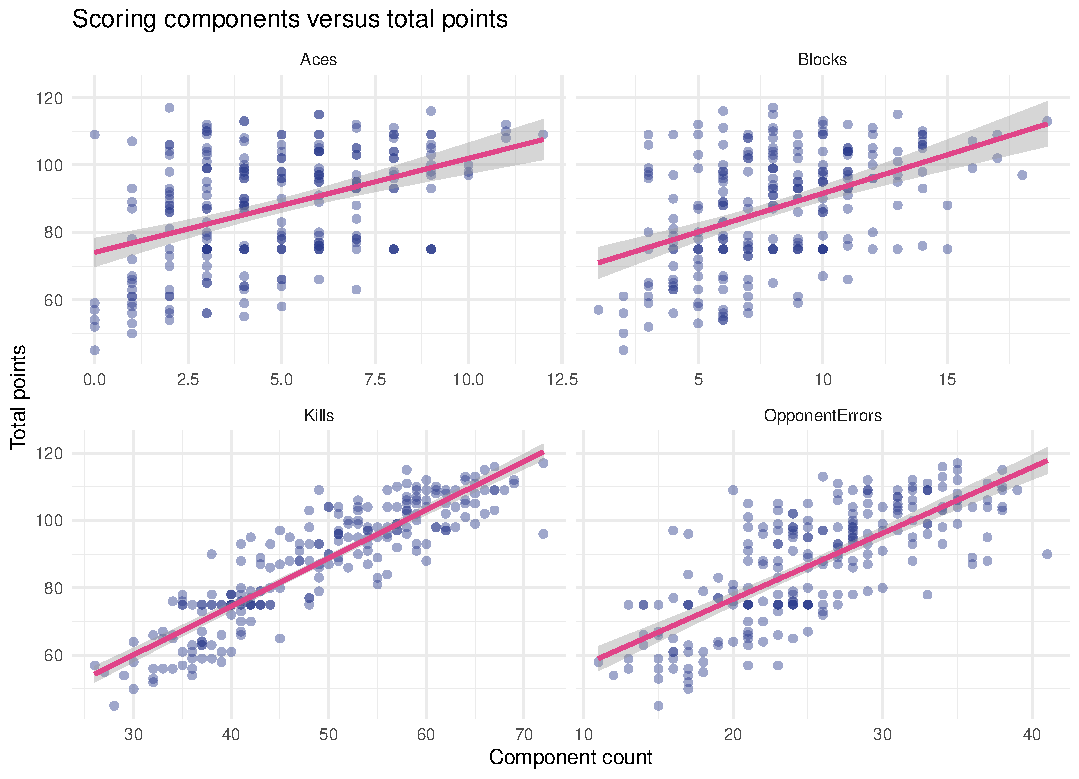
\includegraphics[width=.70\textwidth]{../../outputs/exercise1/scoring_components.pdf}
\caption{Scoring components versus total points; lines are linear fits with 95\% confidence bands.}\label{fig:components}
\end{figure}
\FloatBarrier
\section{Conclusion}
Set-score gaps are explained by match structure, whereas reception missingness is plausibly MCAR under explicit diagnostics. Home total points are non-normal. The data provide no home advantage and show robust away-side differences in kills and total points. The strong kill--total relationship is substantively meaningful but partly exposure-driven.
\section*{Statement of Contributions}
Indudhara Swamy Vivekananda led Exercise 1, including data preparation, missingness assessment, imputation, normality testing, exploratory analysis, visualisation, and the first report draft. Sanjana Basoor Hemanth Kumar and Rohit Mamgin contributed through independent result checking, discussion of interpretations and limitations, integration with the complete case study, proofreading, and final review.
\end{document}

